\documentclass[12pt,a4paper]{article}

\usepackage[UTF8]{ctex}
\usepackage{amsmath,amscd,amsbsy,amssymb,latexsym,url,bm,amsthm}
\usepackage{amsfonts}
\usepackage{epsfig,graphicx,subfigure}
\usepackage{hyperref}
\usepackage{listings}
\usepackage[vlined,ruled,linesnumbered]{algorithm2e}
\usepackage{enumitem}
\usepackage{xcolor}
\usepackage{geometry}

%\uppercase\expandafter{\romannumeral1}:% 罗马数字。

\lstset{
language=Matlab,
keywordstyle= \color{blue!70},
commentstyle= \color{red!50!green!50!blue!50},
breaklines
}%设置listing插入语言

\setlength{\parindent}{0em}
\setlength{\parskip}{1em}

\geometry{bottom =3cm}
\newcommand{\textbi}[1]{%
\textbf{\textit{#1}}}

\newcommand{\ncolor}[1]{%
{\color[RGB]{139,117,0}{#1}}}
\newtheorem{theorem}{Theorem}[section]
\newenvironment{solution}{{\noindent \it \textbf{Solution:}}\\}

\title{MCM daily}
\author{Yunlong Cheng}

\begin{document}
\maketitle
\section{2018-B题-智能RGV动态调度简述}
总共有8台数控机床(CNC), 1辆轨道式自动引导车(RGV), 1条上料带、1条下料带。RGV小车负责“上料,清洗,下料”。

\begin{center}
  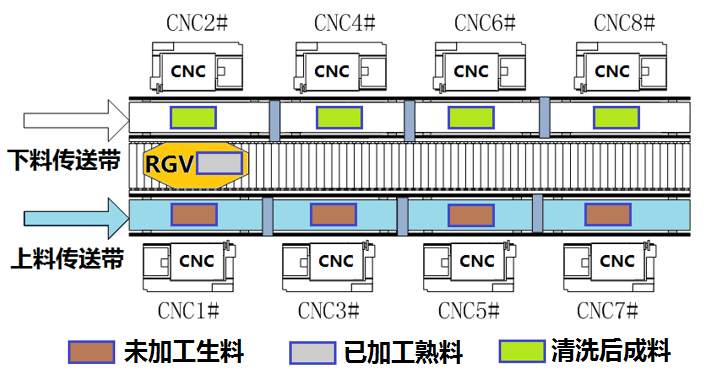
\includegraphics[width = 0.9\textwidth]{figures/illustrate-diagram.png}
\end{center}
针对以下三种情况完成两项任务:
\begin{itemize}
  \item 一道工序的物料加工,物料可以在任一台 CNC 加工。
  \item 两道工序的加工,物料的两道工序分别由不同的 CNC 完成。
  \item CNC 加工可能出现故障,故障排除需要人工完成
\end{itemize}
任务:
\begin{itemize}
  \item 对于一般问题给出 RGV 调度模型和算法。
  \item 利用参数检验模型实用性和算法的有效性,给出RGV调度策略和系统作业效率,并将具体结果填入附件2。
\end{itemize}

\section{分析}


\end{document}
